Plugin del browser Mozilla Firefox, permette di attuare modifiche instantanee sugli stili, le immagini, i form eccetera.\\
Strumento molto utile per capire come viene visualizzata una pagina in caso in cui alcuni elementi non vengano caricati (p.e. come si visualizza l'alt di un'immagine se questa non viene caricata). 
\begin{figure}[!h]
	\centering
	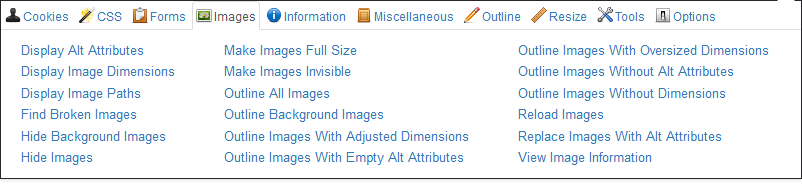
\includegraphics[width=0.7\linewidth]{sezioni/FaseTest/Immagini/web_developer.png}\\
	\caption{Web Developer: Images}
	\label{Fig:webDev}
\end{figure} 